\chapter{提案手法}
発話データの長さにより、i-vectorを抽出精度が大きく異なることが予備実験により明らかである。\par
本研究では2通りの方法で前後の同一話者と考えられる発話区間を結合し、擬似的に長い発話データを作成する。1つ目は発話間の時間情報を考慮した発話区間の結合手法である。2つめは、話者の発話環境を考慮した発話区間の結合手法である。

\section{発話間の時間情報を考慮した発話区間の結合手法}
本手法では、発話区間と発話区間の間(非発話区間)が短い場合、発話区間を結合する。これは図〜で示されるように、同一話者が連続で発話する場合1秒以内に次の発話を行うことが非常に多く、非発話区間が非常に短いためである。つまり、非発話区間が非常に短いとき、高い確率で同一話者の発話区間であることがわかる。しかし、話者が切り替わった場合でも図〜で示されているように、非発話区間が非常に短い場合がある。これは、アンカーと中継アナウンサー、もしくは天気アナウンサーとの会話の中で「はい」「そうですね」など相槌が入るためである。予備実験で非常に短い発話によるi-vectorの誤差は非常に小さいものであることを示した。よって、誤って異なる話者の非常に短い発話区間を結合しても影響は少ないものであると考え、非発話区間が一定時間以内であった場合、前後の発話区間を結合する。

\section{発話環境を考慮した発話区間の結合手法}
本手法では、発話環境の変化を音源識別によって検出し、同一話者の可能性が高い前後の発話区間を結合する。ニュース番組にはスタジオにいるアンカーや天気アナウンサーのほか、台風の状況を中継する中継アナウンサー、騒音の中でインタビューを受けるインタビューイなどが存在する。そこで、アンカーから中継アナウンサー、インタビューイからアンカーなど話者が切り替わった場合発話環境が変化することに着目した。しかし、音源識別では、発話の背景雑音がどの種類であるかを特定することが非常に難しい。そこで、非発話区間の音源識別結果を用いることで、発話環境の変化を検出する。発話環境の変化の検出方法を以下の図に示す。\par

\begin{figure}[htb]
  \begin{center}
    \includegraphics{./figure/piano.eps}
  \end{center}
  \caption{ぴあの}
  \label{fig:one}
\end{figure}


上の例では、最初の話者の非発話区間が「無音区間」であることから、雑音が少ない環境で発話していることがわかる。ここで、次の話者が発話を始めたとき、発話環境が「雑音区間」に変化している。つまり、雑音の多い屋外などで発話をしているインタビューイや中継アナウンサーに話者が切り替わったと考えられる。ここで、前の非発話区間と現在の非発話区間の音源識別結果を参照し、同一の結果であった場合発話区間を結合、異なった場合、話者の切り替わりと識別する。

\begin{figure}[htb]
  \begin{center}
    \includegraphics{./figure/piano.eps}
  \end{center}
  \caption{ぴあの}
  \label{fig:one}
\end{figure}

